\documentclass[serif,mathserif]{beamer}
\usepackage{amsmath, amsfonts, epsfig, xspace}
\usepackage{algorithm,algorithmic}
\usepackage{pstricks,pst-node}
\usepackage{multimedia}
\usepackage{color}
\usepackage[normal,tight,center]{subfigure}
\setlength{\subfigcapskip}{-.5em}
\usepackage{beamerthemesplit}
\usetheme{lankton-keynote}

\author{Agertz et al. 2013, ApJ submitted}

\title[Energy and Momentum From Stellar
Feedback\hspace{2em}\insertframenumber/\inserttotalframenumber]{Towards a
	Complete Accounting of Energy and Momentum from Stellar Feedback in Galaxy
Formation Simulations}

\date{Feb. 28 2013} %leave out for today's date to be insterted

\institute{McMaster Physics \& Astronomy Journal Club}

\begin{document}

\maketitle

\begin{frame}
  \frametitle{Introduction}
  \begin{itemize}
	  \item Why is stellar feedback important?
	  \item Why is stellar feedback hard to model numerically?
	  \item What can we do about it?
	  \item Does any of that actually work?
  \end{itemize}
\end{frame}

\begin{frame}
  \frametitle{What Stellar Feedback Is}
  \begin{itemize}
	  \item Generally: Any processes that transports mass or energy from stars
		  to the ISM
	  \item Specifically: radiation, winds, and supernovae
  \end{itemize}
\end{frame}

\begin{frame}
  \frametitle{What Stellar Feedback Does}
  \begin{itemize}
	  \item Determines SFR \& SFH
	  \item Creates the Kennicutt-Schmidt Law
	  \item Sets the $M_*/M_b$ fraction
	  \item Destroys GMCs
	  \item Turns cusps into cores 
	  \item Powers fountains and outflows
	  \item Drives 3-phase instability (McKee \& Ostriker 1977 Model)
  \end{itemize}
\end{frame}

\begin{frame}
  \frametitle{What Stellar Feedback Does}
  \begin{itemize}
	  \item {\color{red} Determines SFR \& SFH}
	  \item {\color{red} Creates the Kennicutt-Schmidt Law}
	  \item {\color{red} Sets the $M_*/M_b$ fraction}
	  \item Destroys GMCs
	  \item Turns cusps into cores 
	  \item Powers fountains and outflows
	  \item Drives 3-phase instability (McKee \& Ostriker 1977 Model)
  \end{itemize}
\end{frame}

\begin{frame}
	\frametitle{Stellar Feedback Is Not A New Idea}
	\begin{figure}[t]
	\centering
	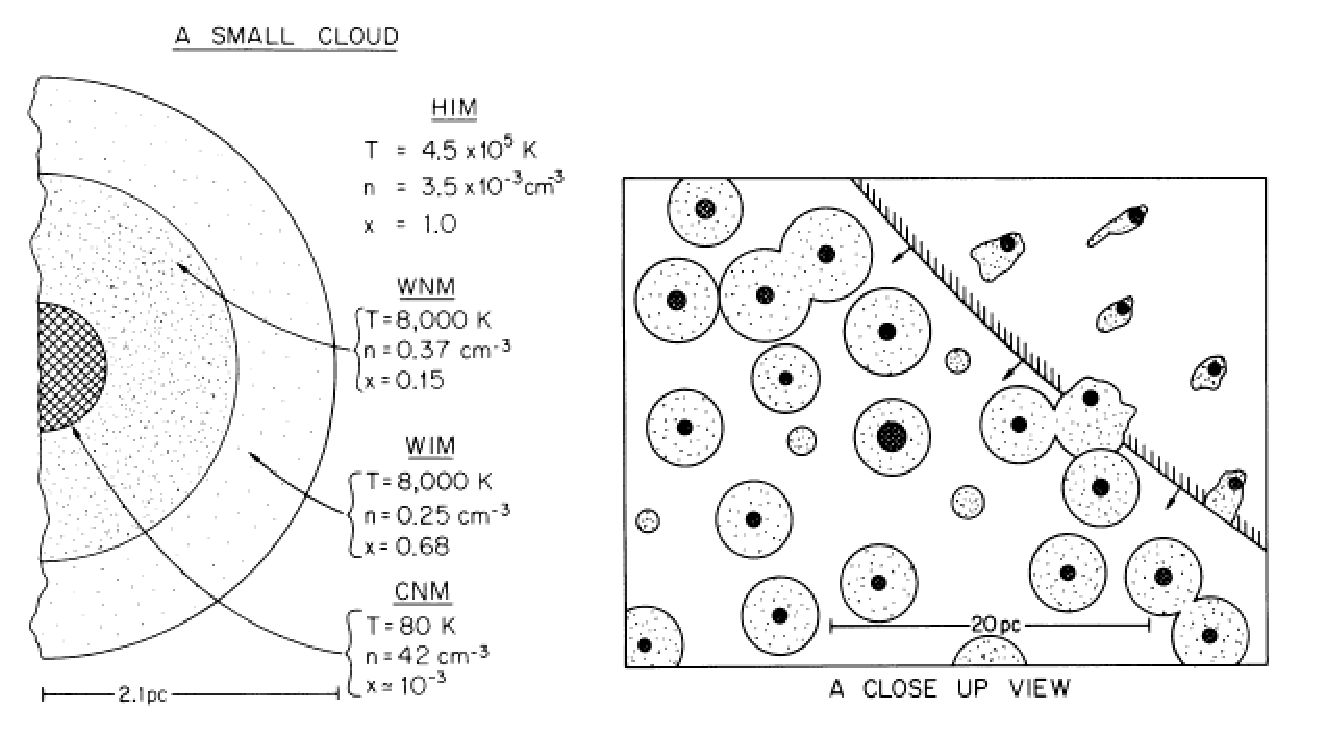
\includegraphics[width=6.5cm]{figures/mckee_ostriker1}
	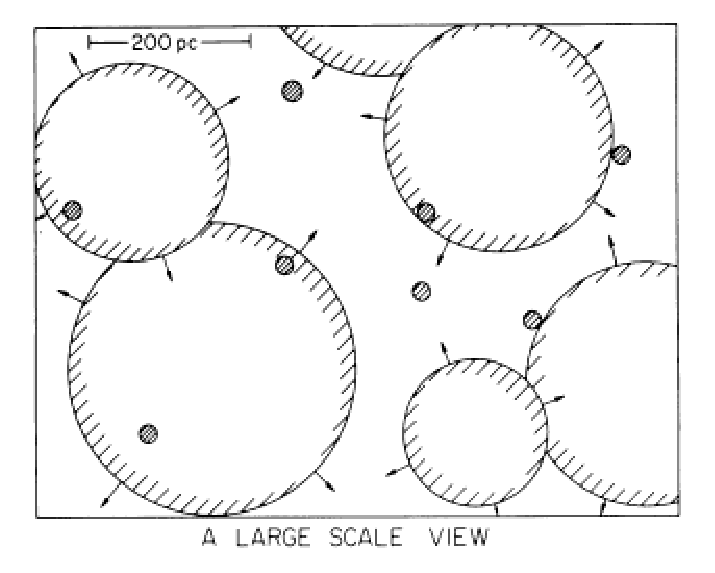
\includegraphics[width=5cm]{figures/mckee_ostriker2}\\
	\tiny{McKee \& Ostriker 1977}
	\end{figure}
\end{frame}

\begin{frame}
	\frametitle{How Much Energy Is In Feedback}
	\begin{figure}[t]
	\centering
	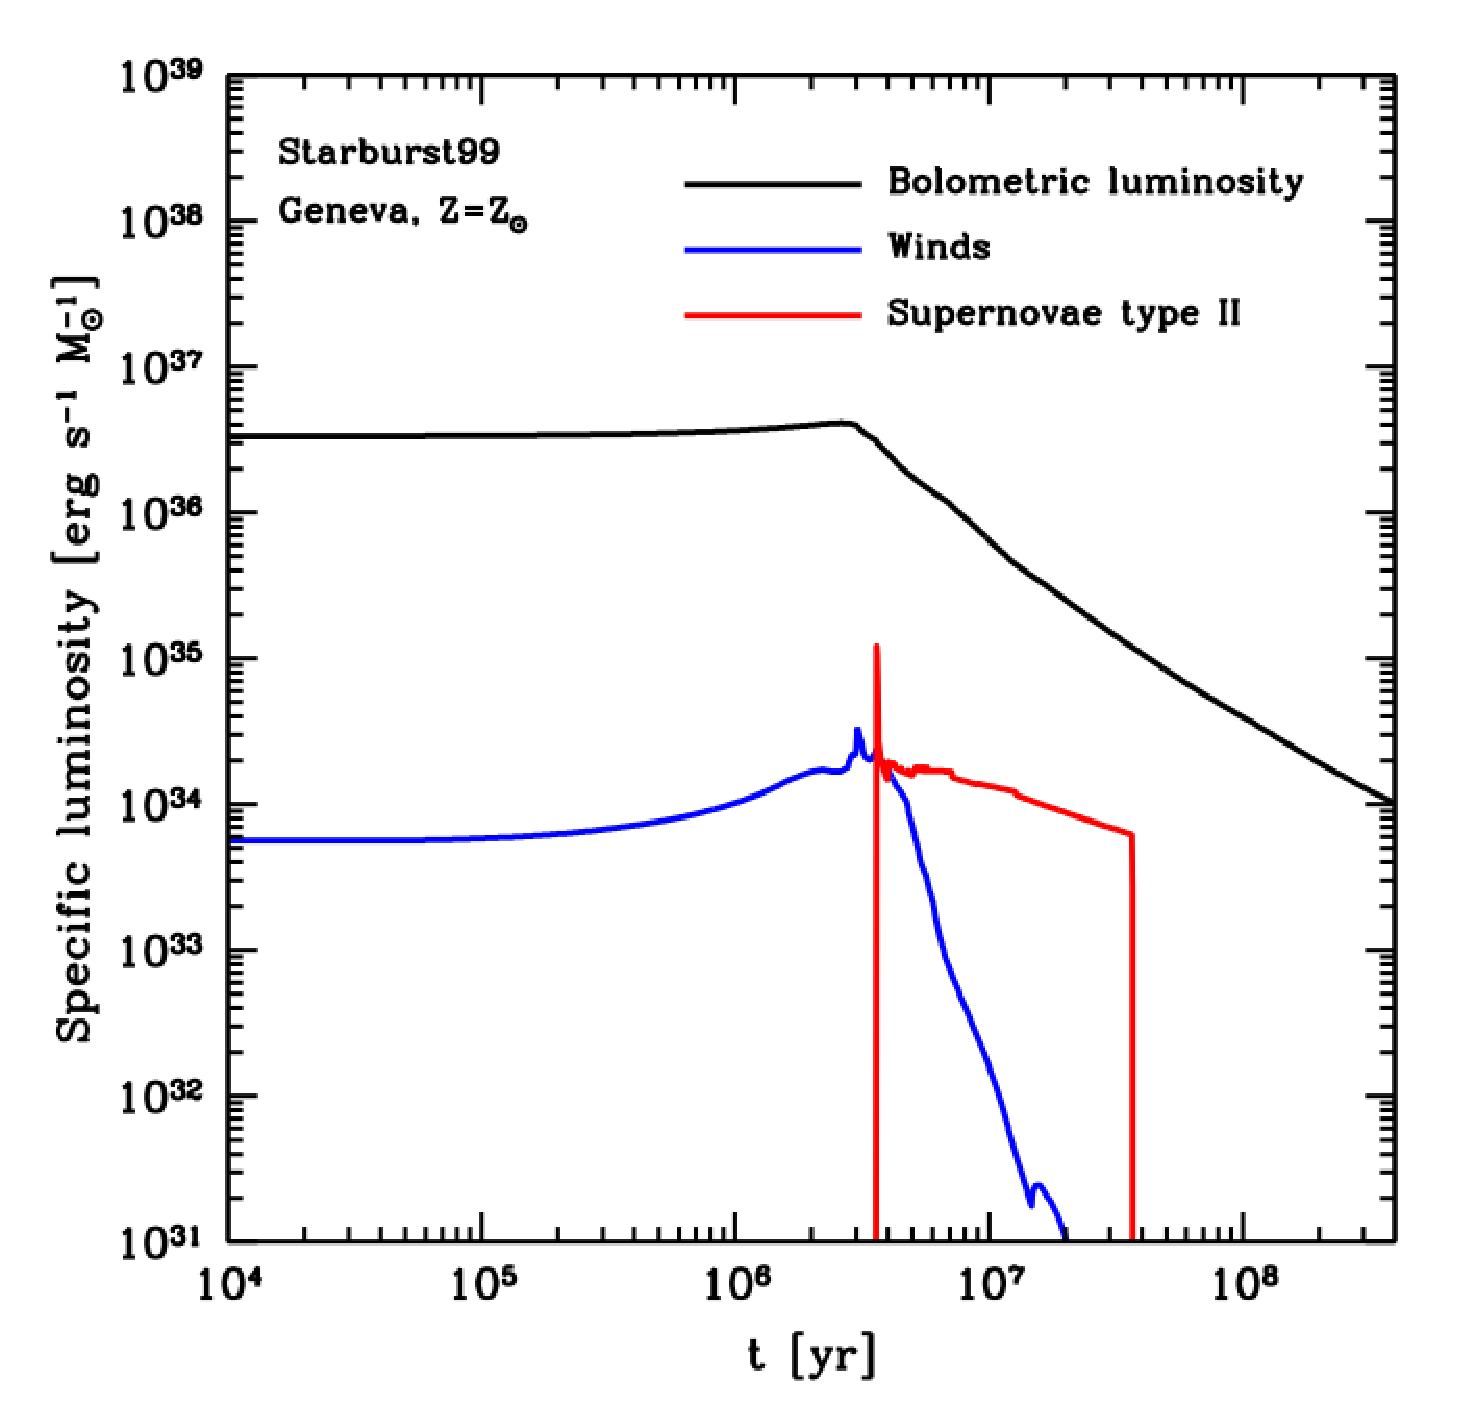
\includegraphics[width=8cm]{figures/SB99_luminosity}\\
	\tiny{Agertz et al. 2013}
	\end{figure}
\end{frame}

\begin{frame}
	\frametitle{How Does The Energy Get Out}
	\begin{columns}[c]
		\column{.5\textwidth}
		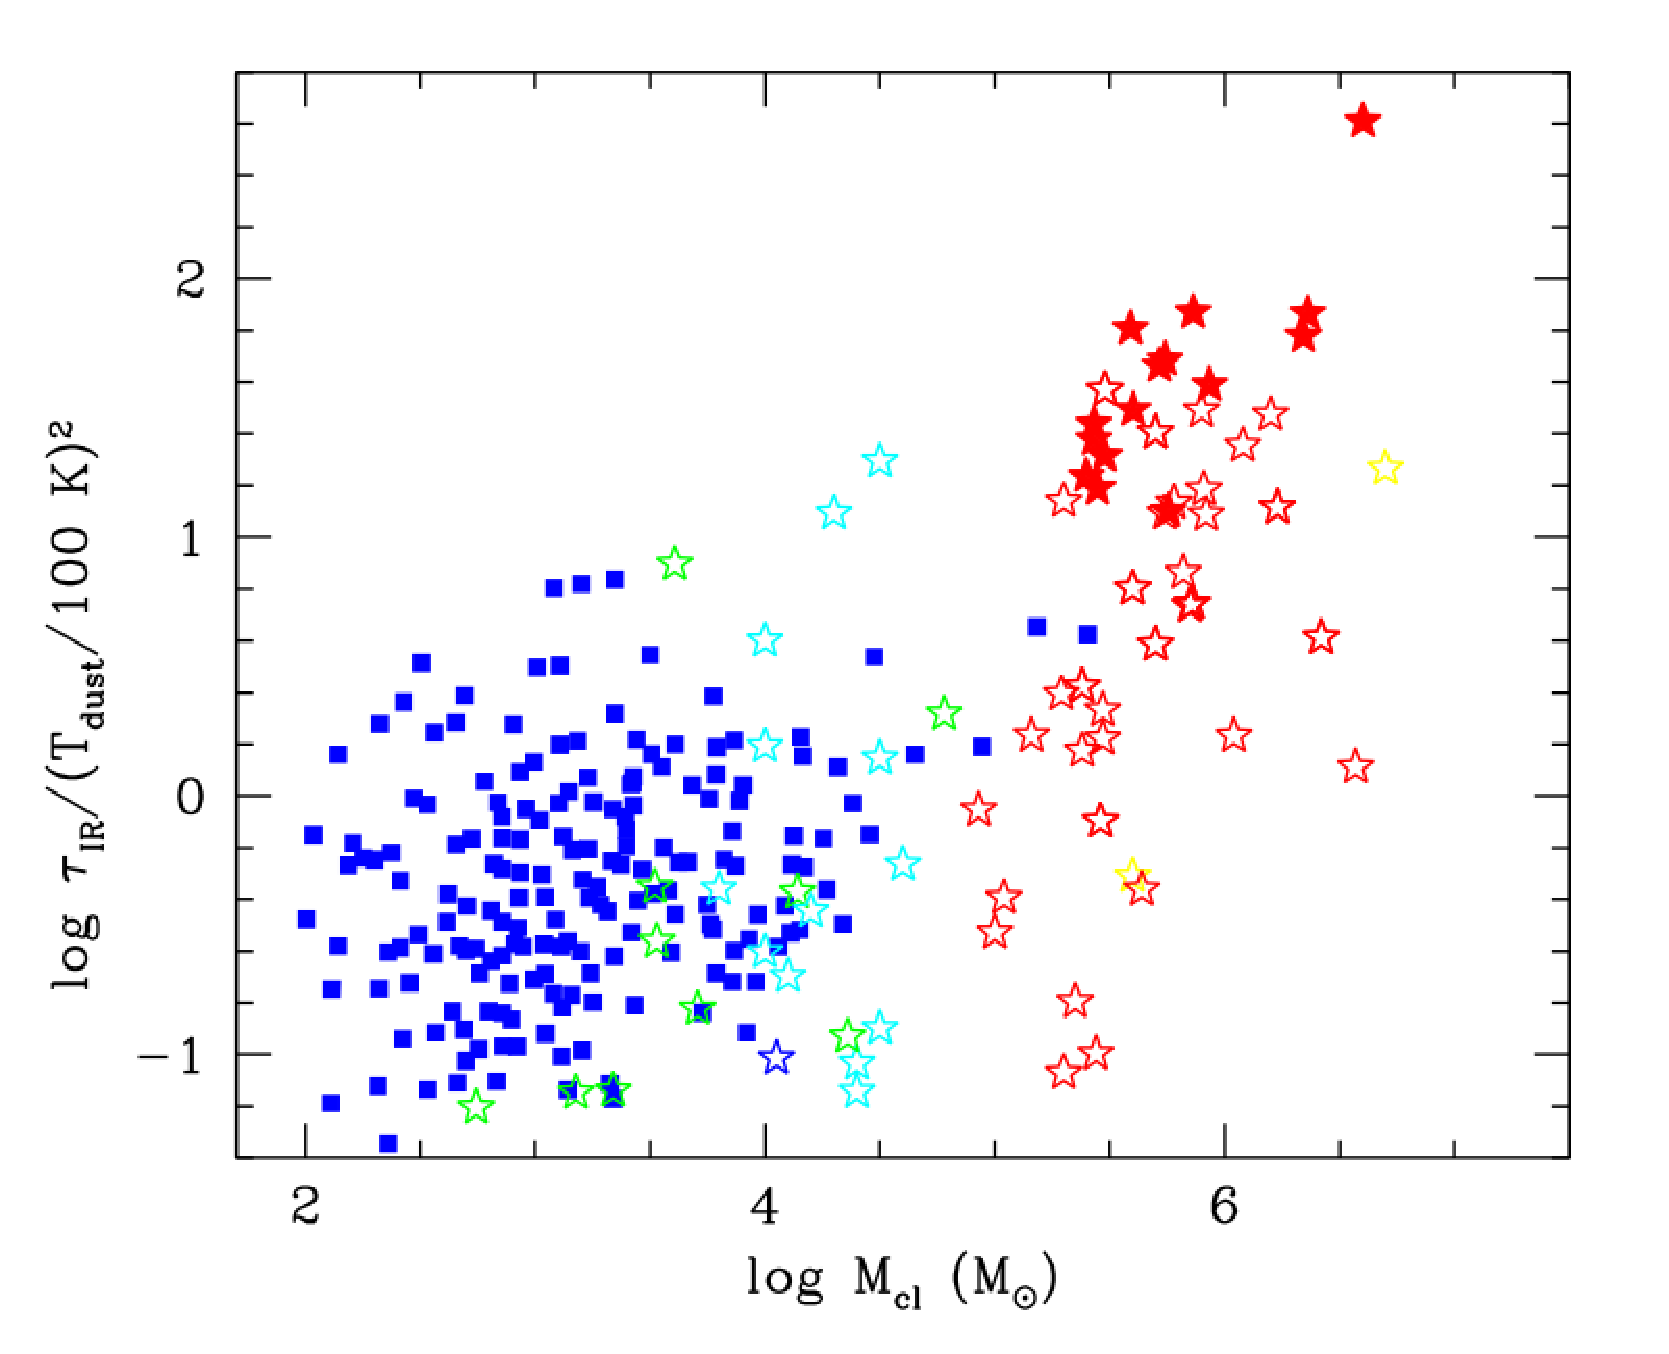
\includegraphics[width=5cm]{figures/opticaldepth}\\
		\tiny{Agertz et al. 2013}
		\column{.5\textwidth}
		\begin{itemize}
			\item Stellar Winds
				\begin{itemize}
					\item Massive Stars drive $\approx 10^3 km/s$ winds
				\end{itemize}
			\item Radiation Pressure $\dot p_{rad} = (\eta_1+\eta_2\tau_{IR})\frac{L(t)}{c}$
			\item Supernovae
				\begin{itemize}
					\item Type II and Ia
					\item 3 Stages:
					\begin{itemize}
						\item Ballistic
						\item Adiabatic
						\item Isothermal
					\end{itemize}
				\end{itemize}
			\item AGB Mass Loss
		\end{itemize}
	\end{columns}
\end{frame}

\begin{frame}
	\frametitle{Why It Is Difficult To Implement}
	\begin{itemize}
		\item Resolution
		\item Resolution
		\item Did I mention resolution?
		\item Also uncertain physics
	\end{itemize}
\end{frame}

\begin{frame}
	\frametitle{Typical Simulation Resolutions}
	\begin{columns}[c]
		\column{.5\textwidth}
	\begin{itemize}
		\item $\Delta M \approx 10^2-10^3 M_\odot$
		\item $\Delta L \approx 10-100 pc$
		\item $\Delta t \approx 0.1\frac{\Delta L}{v}$
	\end{itemize}
		\column{.5\textwidth}
		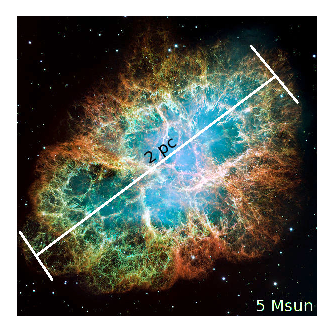
\includegraphics[width=5cm]{figures/crab}\\
		\tiny{hubblesite.org}
	\end{columns}
\end{frame}

\begin{frame}
	\frametitle{Naive Feedback}
	\begin{itemize}
		\item Deposit feedback energy $\epsilon_{FB}$ as heat either instantaneously or
			continuously into a few $N$ resolution elements, with a mass $NM_p$
		\item One feedback event will raise the temperature in this gas by
			$\Delta T = \frac{2}{3k_B}\epsilon_{FB}\frac{NM_p}{m_H}$
	\end{itemize}
\end{frame}

\begin{frame}
	\frametitle{Overcooling}
	\begin{figure}[t]
	\centering
	\includegraphics[width=7cm]{figures/Thacker_Couchman}\\
	\tiny{Thacker \& Couchman 2000}
	\end{figure}
\end{frame}

\begin{frame}
	\frametitle{What makes a good model}
	\begin{columns}[c]
		\column{.5\textwidth}
		\begin{itemize}
			\item Works for very unresolved feedback (subgrid)
			\item Little/no resolution dependence
			\item Few, well constrained/motivated parameters
		\end{itemize}
		\column{.5\textwidth}
			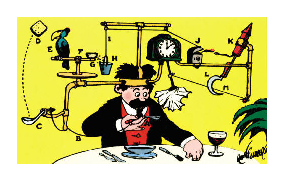
\includegraphics[width=6cm]{figures/rube}\\
			\tiny{Goldberg 1995}
	\end{columns}
\end{frame}

\begin{frame}
	\frametitle{What makes this model}
	\begin{itemize}
		\item Energy: $E = E_{SNII}+E_{SNIa}+E_{wind}$
		\item Momentum: $p = p_{SNII}+p_{rad}+E_{wind}$
		\item Mass Loss: $m = m_{SNII}+m_{SNIa}+m_{wind}+m_{loss}$
		\item Metal Enrichment: $m_Z = m_{Z,SNII}+m_{Z,SNIa}+m_{Z,wind}+m_{Z,loss}$
	\end{itemize}
\end{frame}

\begin{frame}
	\frametitle{Type II \& Ia Supernovae}
	\begin{itemize}
		\item Number Determined by IMF $N_{SNII}$ 
		\item Energy based on an average SNII energy $N_{SNII}10^{51}erg$ 
		\item Momentum based on ejected mass ($12 M_\odot$) and ejecta 
			velocity ($3000 km/s$)\\$p_{SNII} =
			N_{SNII}m_{ej}v_{ej}$ (This could be much higher if the adiabatic
			phase is included)
		\item Type Ia supernova Eject much less mass, so they do not contribute
			significantly to momentum flux
		\item Cooling shutoff: Adiabatic phase
	\end{itemize}
\end{frame}

\begin{frame}
	\frametitle{Radiation, Winds, Mass Loss}
	\begin{itemize}
		\item Winds approximated using a fit to calculations from Lietherer et
			al. 1992 \& STARBURST99
		\item Radiation pressure approximated using gas surface density
			(Calculating optical depth is VERY EXPENSIVE)
	\end{itemize}
			\includegraphics[width=10cm]{figures/energy_momentum_budget}\\
			\tiny{Agertz et al. 2013}
\end{frame}

\begin{frame}
	\frametitle{How well does this perform}
	Isolated Cloud
	\begin{figure}[t]
	\centering
	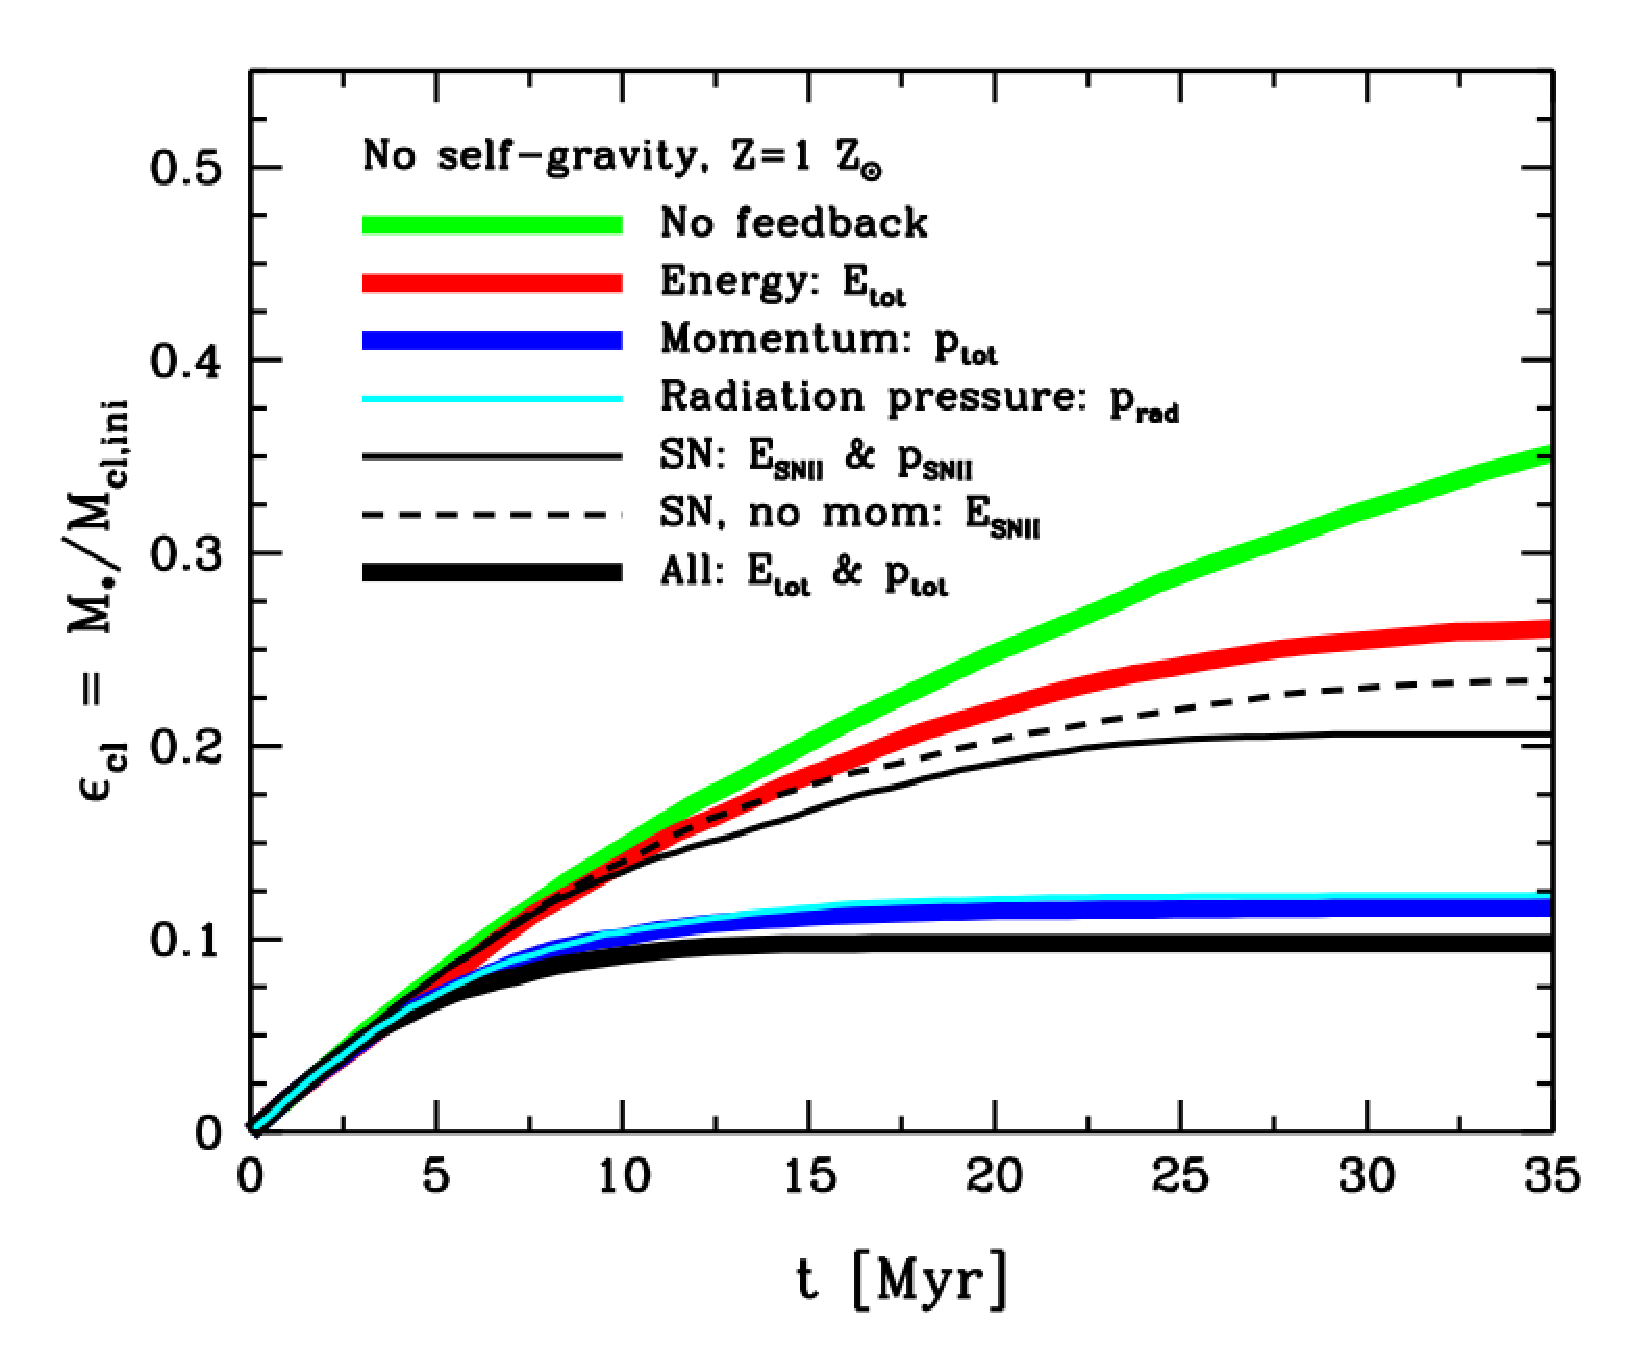
\includegraphics[width=7cm]{figures/cloud}\\
	\tiny{Agertz et al. 2013}
	\end{figure}
\end{frame}


\begin{frame}
	\frametitle{How well does this perform}
	Isolated Galaxy
	\begin{figure}[t]
	\centering
	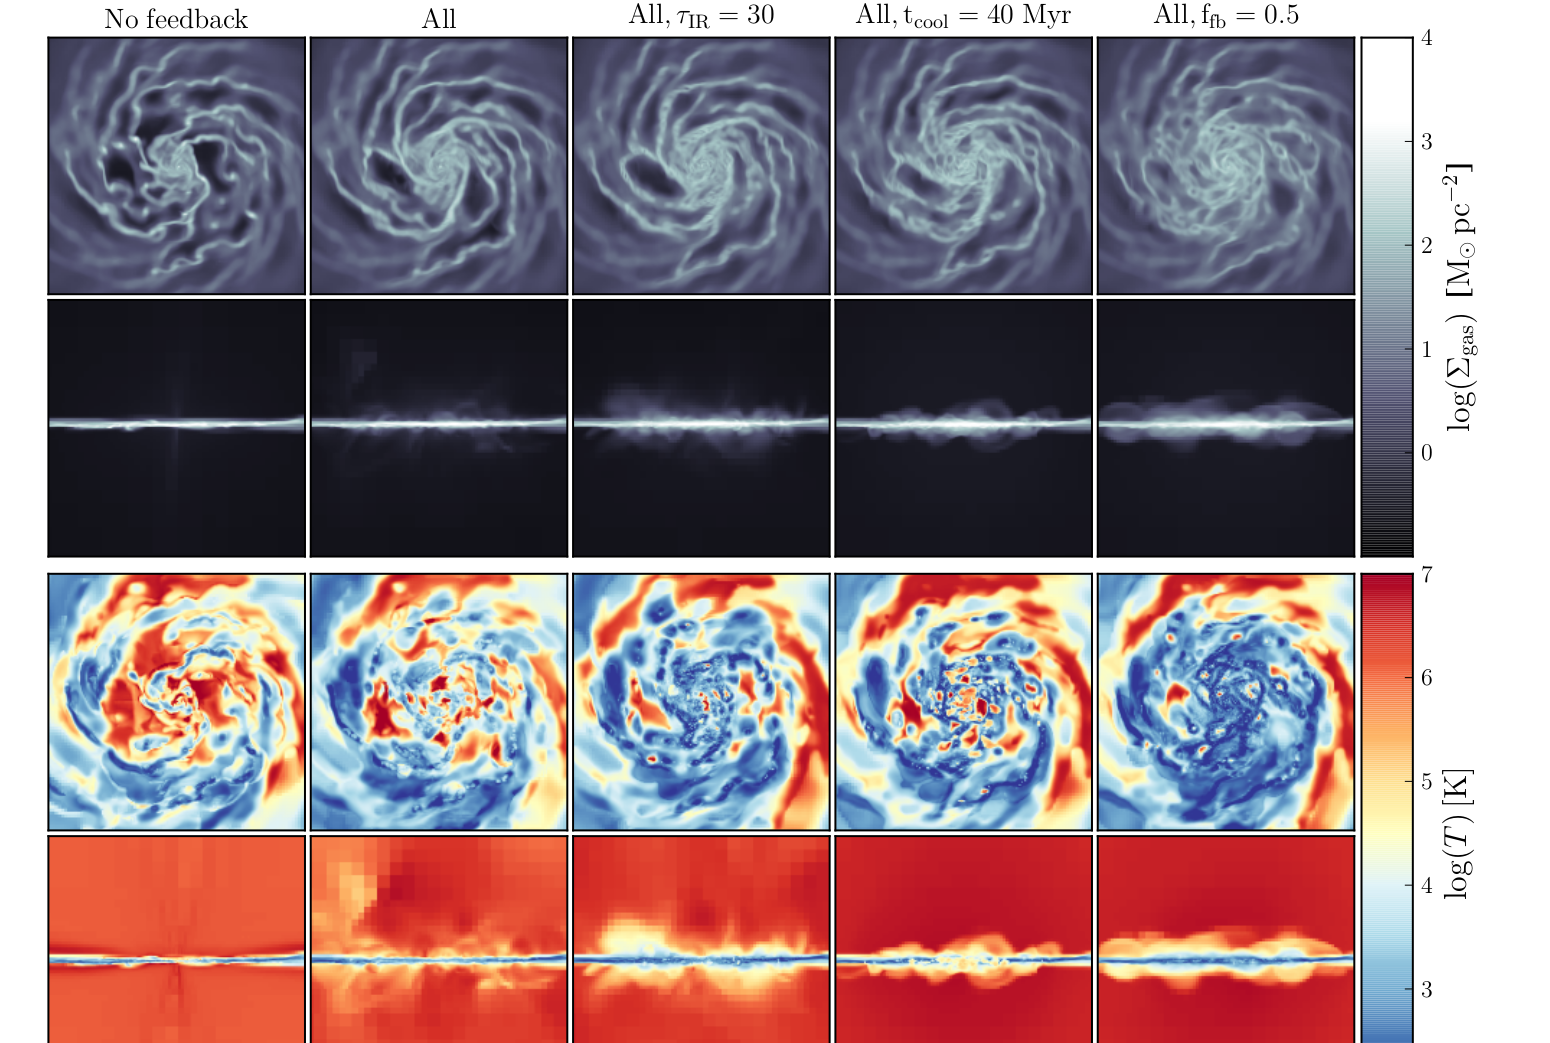
\includegraphics[width=9cm]{figures/galaxy}\\
	\tiny{Agertz et al. 2013}
	\end{figure}
\end{frame}

\begin{frame}
	\frametitle{How well does this perform}
	Star Formation History
	\begin{figure}[t]
	\centering
	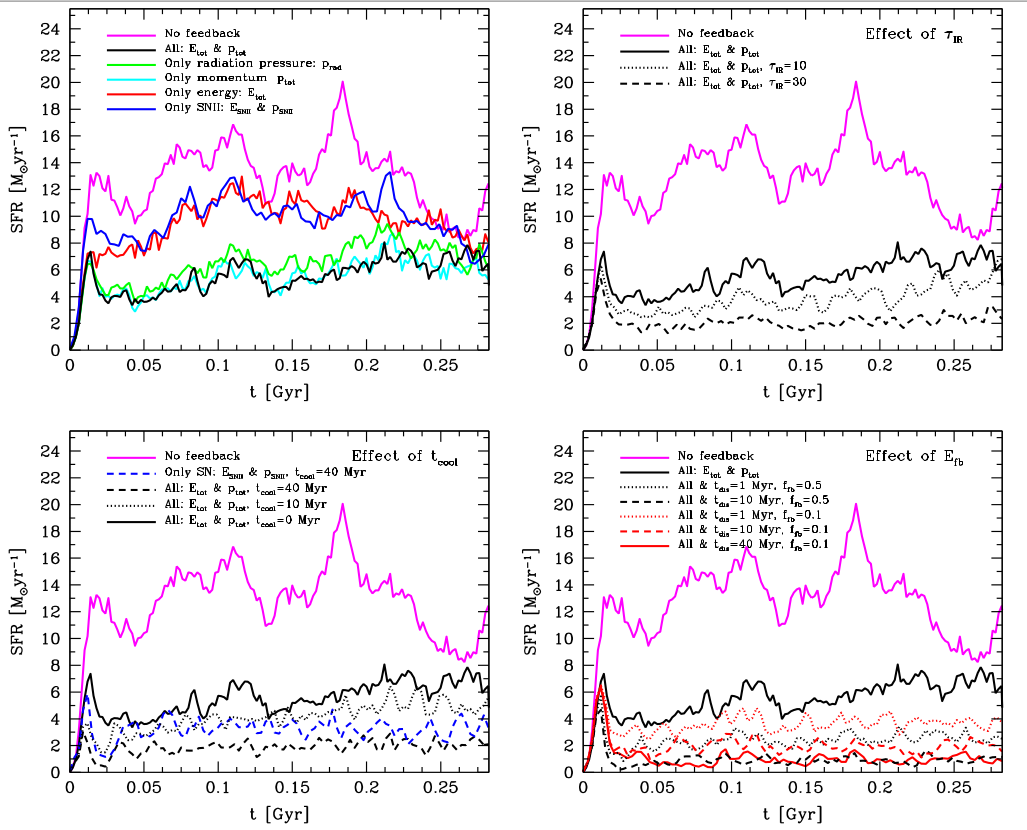
\includegraphics[width=8.5cm]{figures/SFR}\\
	\tiny{Agertz et al. 2013}
	\end{figure}
\end{frame}

\begin{frame}
	\frametitle{How well does this perform}
	Kennicutt Law
	\begin{figure}[t]
	\centering
	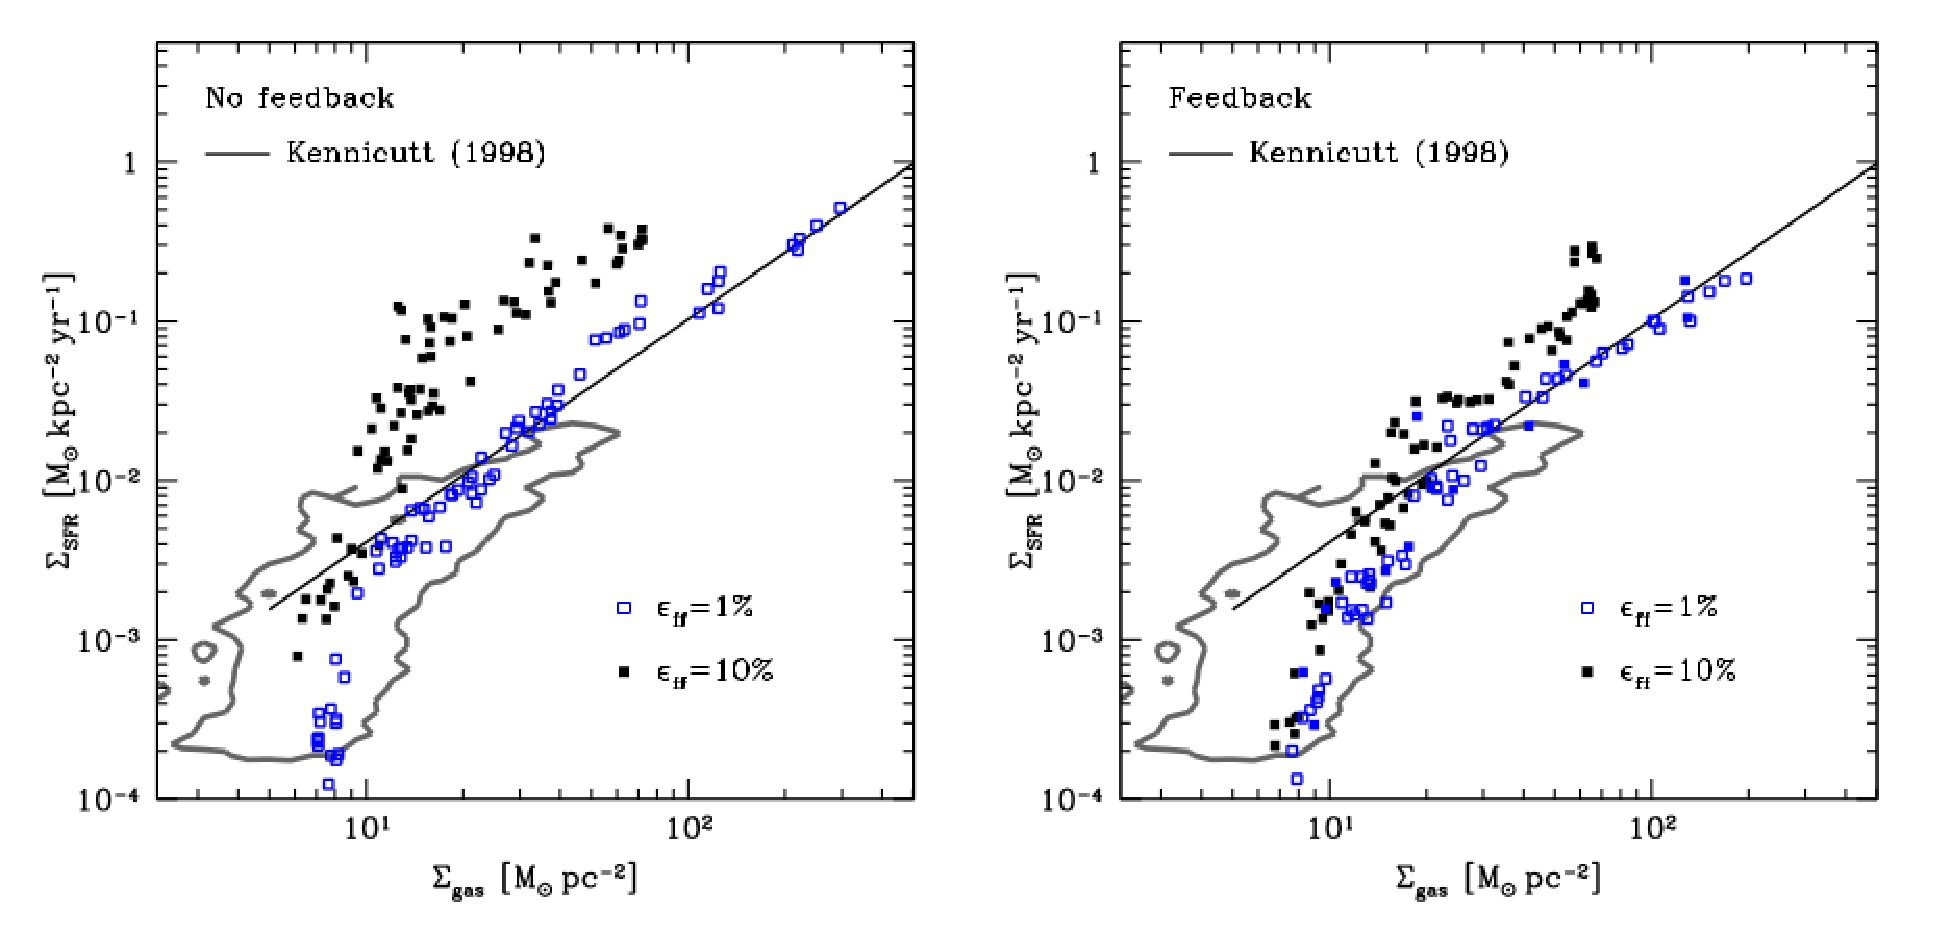
\includegraphics[width=10cm]{figures/Kennicutt}\\
	\tiny{Agertz et al. 2013}
	\end{figure}
\end{frame}

\begin{frame}
	\frametitle{Take Away Message}
	\begin{itemize}
		\item Removing numerical effects in feedback models is essential, extremely difficult
		\item Feedback models need good observation constraints for both
			parameters and effects
		\item We aren't done yet.
	\end{itemize}
\end{frame}
\end{document}
